\chapter{Постановка задачи}\label{ch:ch1}
\section{Обзор робота}\label{sec:ch1/sec1}
В данной задаче используется робот, собранный из сервомоторов Kondo и неподвыжных частей (рисунок ~\cref{fig:real_robot}). Каждый сервомотор обеспечивает поворот вдоль заданной оси в заданном интервале углов. Движение может происходить как по часовой стрелке, так и против. Для каждого мотора задаётся свой интервал углов, чтобы избегать повреждения робота вследствие самопересечения конструкции робота.

\begin{figure}[ht]
    \centerfloat{
        \label{fig:real_robot-1}}{%
            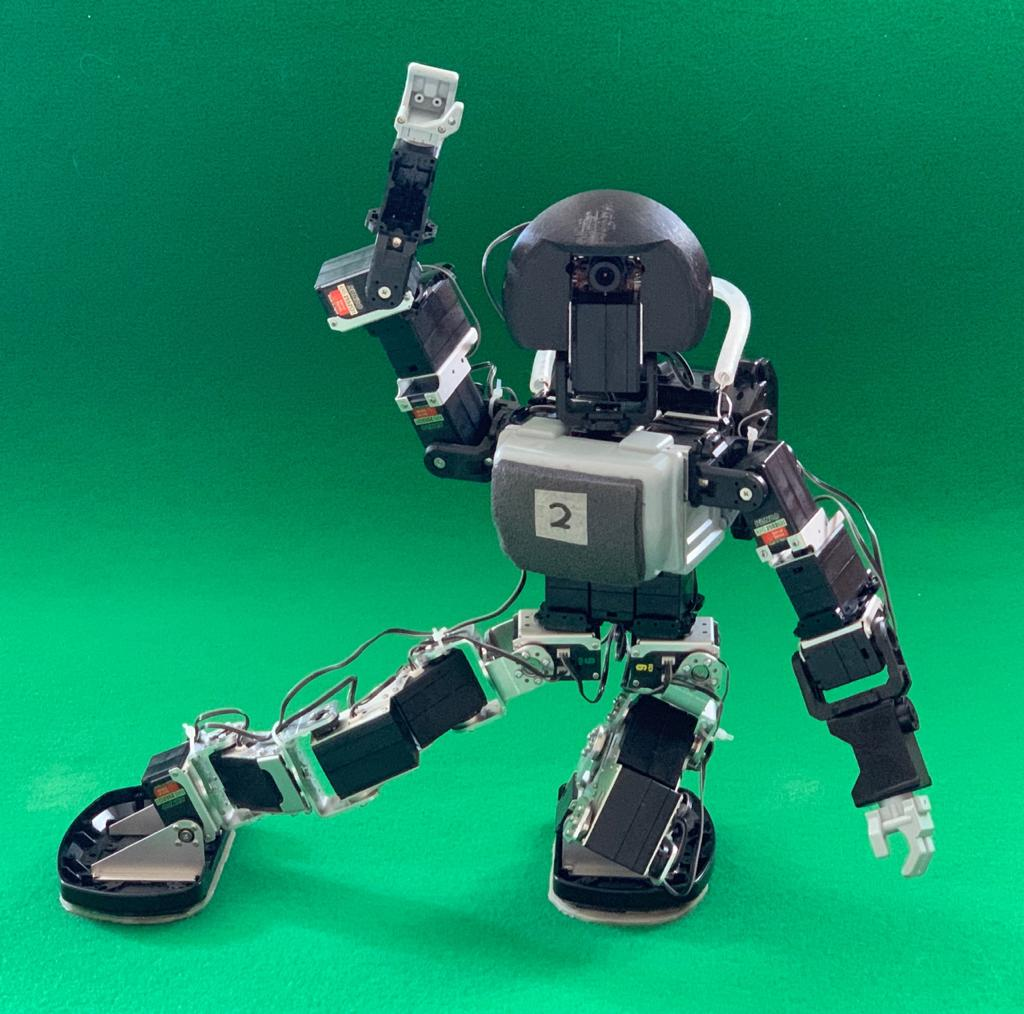
\includegraphics[width=0.5\linewidth]{real_robot}}
    \caption[Изображение робота в действии]{Изображение робота в действии}\label{fig:real_robot}
\end{figure}
\section{Используемый симулятор}\label{sec:ch1/sec1}
